%------------------------------------- CONFIGURAÇÕES DE CAPA --------------------------------------
% TODO: Mudar título
\begin{titlepage}
	% Capa Principal
	\begin{center}
		\Huge{UNIVERSIDADE DE SÃO PAULO}\\
		\vspace{0.02\textheight}
		\huge{ESCOLA DE ENGENHARIA DE SÃO CARLOS}\\
		\vspace{0.01\textheight}
		\huge{DEPARTAMENTO DE ENGENHARIA ELÉTRICA}\\
		\vspace{0.2\textheight}
		\huge{\textbf{Mapeamento de ambientes baseado em algoritmos de visão estéreo para VANTs sobre Linux Embarcado}}
		\vspace{0.2\textheight}
	\end{center}
		
		\large
		{
			\begin{flushleft}
			\Large{ \textbf{Autor}: \hspace{1cm} Nícolas dos Santos Rosa}\\
			\Large{ \textbf{Orientador}: \hspace{0.3cm} Prof. Dr. Evandro Luís Linhari Rodrigues }\\
			\end{flushleft}
	
			\begin{center}
				\vspace{0.09\textheight}
				\Large{São Carlos}\\
				\Large{2016}
			\end{center}
		}
	
\end{titlepage}


%------------------------------------- INSERÇÃO PÁGINA EM BRANCO ------------------------------------
\cleardoublepage

%------------------------------------- FOLHA DE ROSTO  ----------------------------------------------
%\vspace{0.01\textheight} 
	\begin{center}
	\vspace{-0.06\textheight}
	%\thispagestyle{empty}
		\Large{\textbf{Nícolas dos Santos Rosa}}\\
		\vspace{0.15\textheight}
		\Huge{\textbf{Mapeamento de ambientes baseado em algoritmos de visão estéreo para VANTs sobre Linux Embarcado}} 
		\vspace{0.08\textheight}
	\end{center}
		
		\large
		{
			\begin{flushright}
			\Large{Trabalho de Conclusão de Curso apresentado} \hspace{1cm}\\
			\Large{à Escola de Engenharia de São Carlos, da}\\
			\Large{Universidade de São Paulo}\\
			\vspace{0.05\textheight}
			\Large{Curso de Engenharia Elétrica}\\
			\vspace{0.05\textheight}
			\Large{ORIENTADOR: Prof. Evandro Luís Linhari Rodrigues}\\
			\end{flushright}
	
			\begin{center}
				\vspace{0.15\textheight}
				\Large{São Carlos}\\
				\Large{2016}
			\end{center}
		}



%------------------------------------- FICHA CATALOGRÁFICA ------------------------------------------
\newpage

Página com a ficha catalográfica (em página par).

%ficha catalografica no verso
%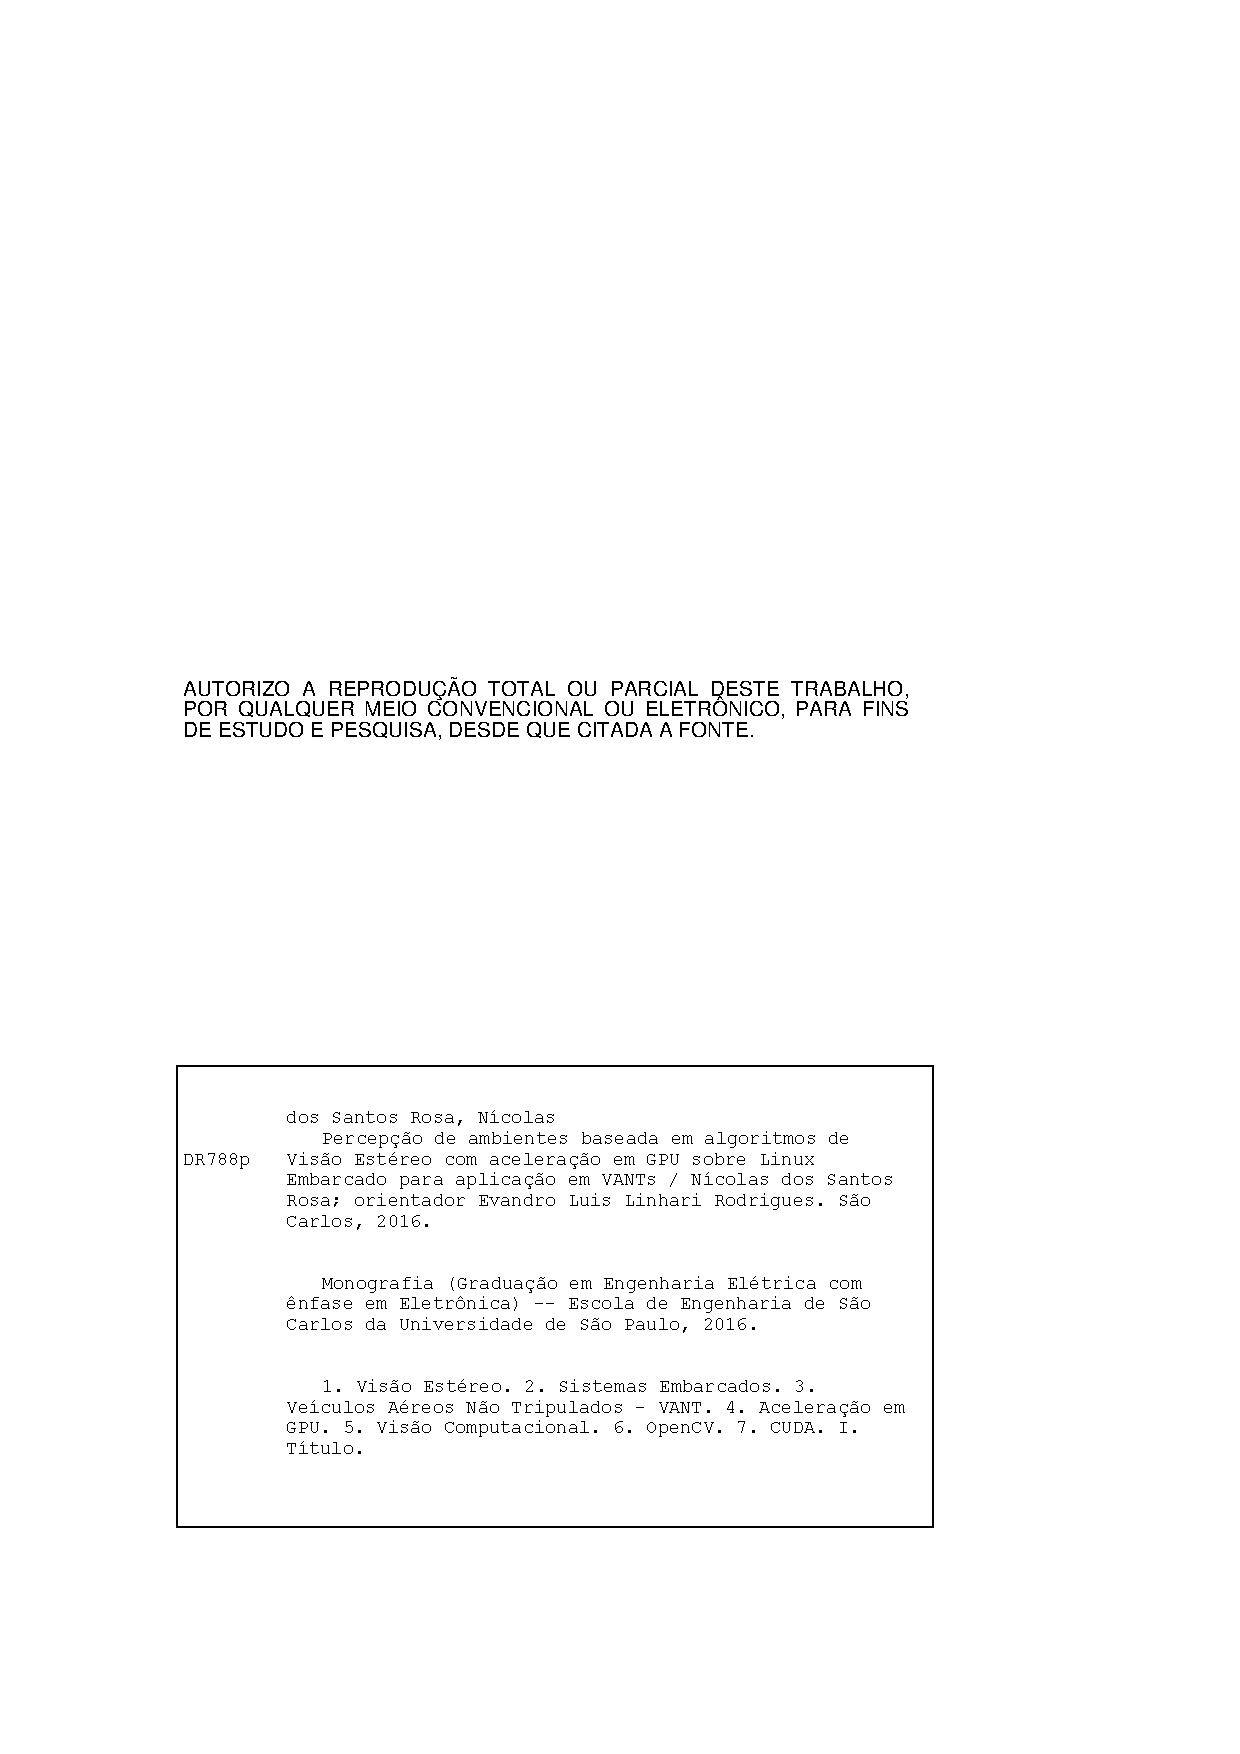
\includepdf{./Resources/ficha_catalografica.pdf}

%------------------------------------- Folha de aprovação--------------------------------------------
\newpage

página com a folha de aprovação (página ímpar). \cleardoublepage

\begin{comment}
\begin{figure}[H]
	\centering
	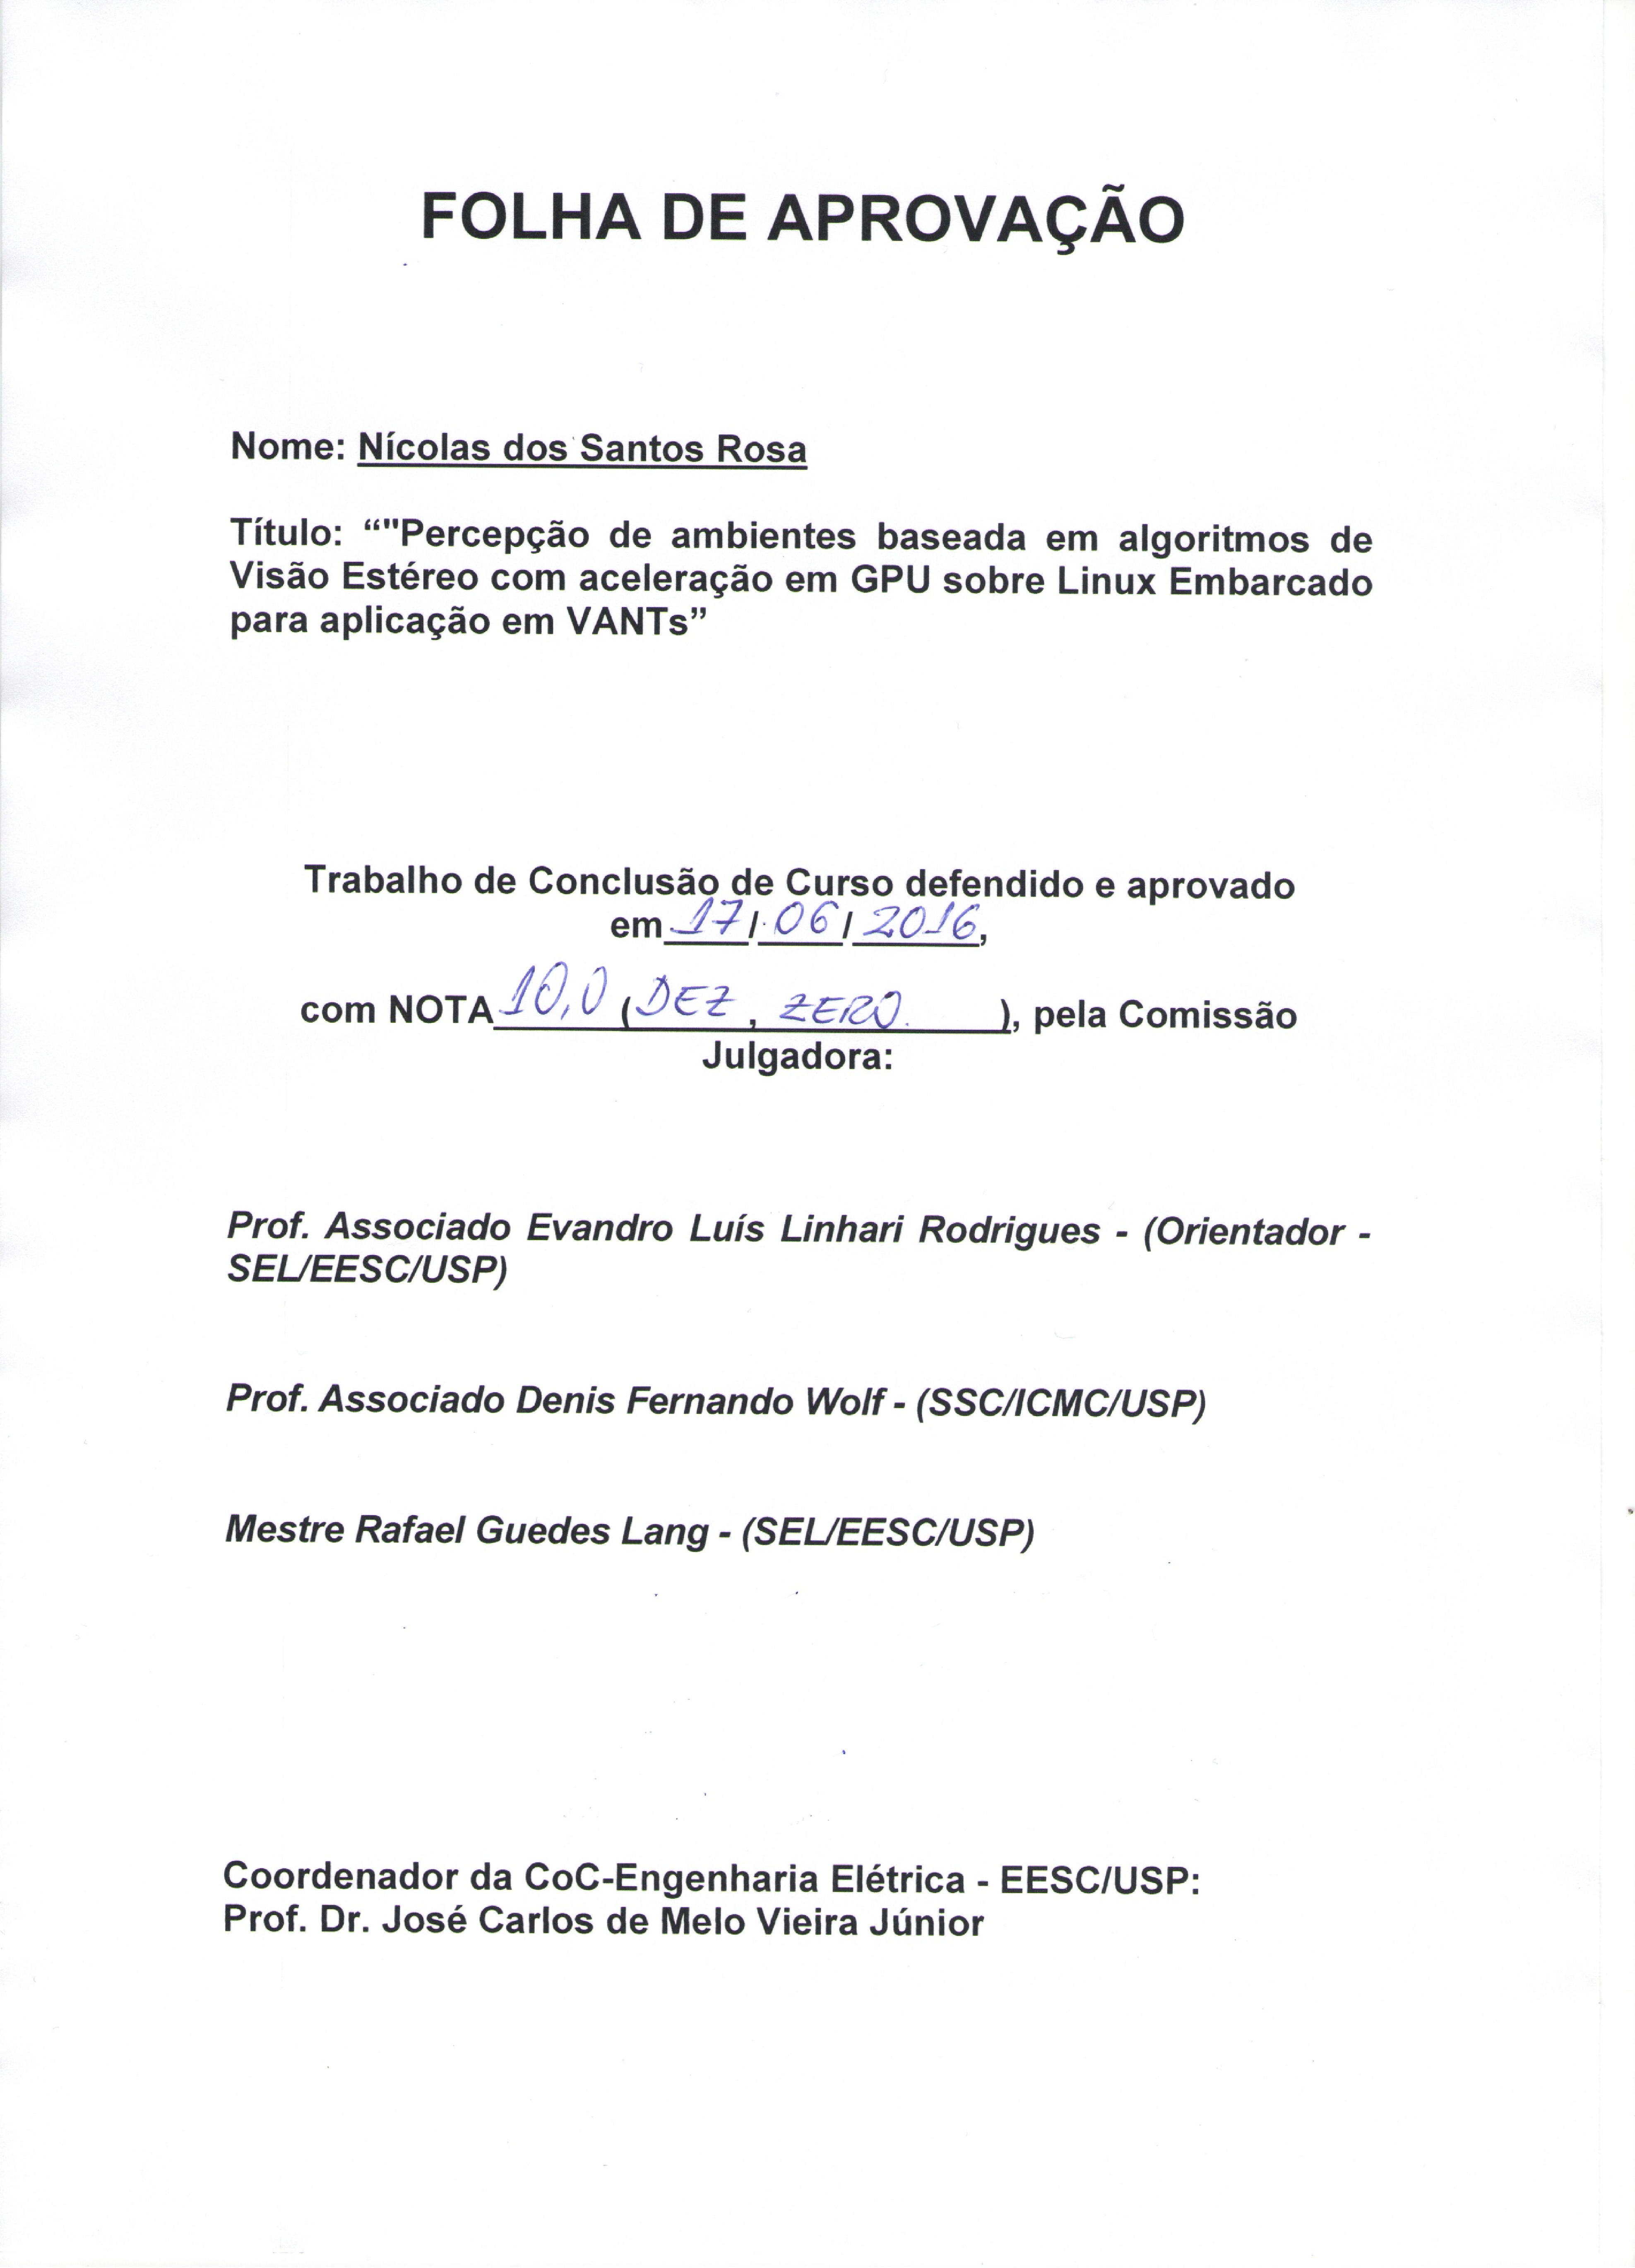
\includegraphics[scale=0.3]{./Resources/aprovacao.jpg}
	\caption{Fluxo de comunicação entre os principais componentes.}
	\label{Aprovacao}
\end{figure}
\cleardoublepage
\end{comment}
%------------------------------------- Dedicatória --------------------------------------------------
\vspace{0.11\textheight} 
\begin{center}
\textbf{\Huge{Dedicatória}}
\end{center}
\vspace{0.05\textheight}

Este trabalho de conclusão de curso é dedicado à minha mãe, ao meu pai, à minha irmã, aos meus padrinhos e a toda minha família.

\begin{flushright}
Nícolas dos Santos Rosa.
\end{flushright}

%------------------------------------- INSERÇÃO PÁGINA EM BRANCO ------------------------------------
\cleardoublepage

%------------------------------------- Agradecimentos -----------------------------------------------
\vspace{0.11\textheight} 

\begin{center}
\textbf{\Huge{Agradecimentos}}
\end{center}

\vspace{0.05\textheight}

Primeiramente, agradeço a Deus por propiciar saúde e felicidade a todos aqueles que me rodeiam.

À minha família: à minha mãe, Valdenilce, pela ferrenha dedicação em mostrar a mim e a minha irmã a importância da educação para nossa formação pessoal; ao meu pai, Francisco, por fazer o possível e o impossível para sustentar nossa família e por possibilitar condições para que me tornasse engenheiro; à minha irmã, Natália, pelo suporte e carinho e por ser a dupla perfeita para atazanar nossos pais; às minhas tias, Elisabeth, Vera Lúcia e Maria Regina, por serem minhas segundas mães, visto o tamanho do suporte, preocupação, e apreço dado. 

Ao meu orientador, Prof. Evandro Luís Linhari Rodrigues, pelo apoio para o desenvolvimento deste trabalho e por despertar meu interesse em sistemas embarcados, confirmando ainda mais minha paixão pelo meu curso.  

Aos meus orientadores de iniciação científica, Prof. Dr. Cláudio F. M. Toledo e Márcio S. Arantes, por introduzir-me ao âmbito da pesquisa acadêmica. Aos membros do SARLab: ao Prof. Dr. Samir Rawashdeh por ser o idealizador deste trabalho e por oferecer a oportunidade de desenvolvê-lo; a Benjamin Dale e a Miguel Rocha Jr., pelo companheirismo e por sempre estarem sempre de prontidão.

Aos meus amigos de curso, pelos ótimos momentos que vivemos juntos nestes anos, especialmente, Alexandre B. Moretti, Leonardo B. Farçoni, Plínio G. B. Ferreira, Marília L. Dourado,  Jéssica B. da Vida, Pedro Arantes, Augusto Martins, Gustavo Oliveira, Aline Midori, Vitor Martins, Anderson M. Tsai, Victor Morini, João F. Corsini, Caio Martins e a todos os outros amigos. 

Aos membros do grupo extracurricular Warthog Robotics, por partilhar um interesse em comum e pelas incontáveis horas de dedicação gastas no laboratório.

Por fim, agradeço a todos os envolvidos no desenvolvimento deste trabalho.

\begin{flushright}
Nícolas dos Santos Rosa.
\end{flushright}


%------------------------------------- INSERÇÃO PÁGINA EM BRANCO ------------------------------------
\cleardoublepage

%------------------------------------- EPÍGRAFE -----------------------------------------------------
\
\vspace{0.76\textheight} 

\begin{flushright}

\textit{"O dinheiro faz homens ricos, o conhecimento faz homens }

\textit{sábios e a humildade faz grandes homens."}

Mahatma Gandhi

\textit{"You can't put a limit on anything. The more you dream, the farther you get."}

Michael Phelps

\textit{"Se eu vi mais longe, foi por estar sobre ombros de gigantes."}

Isaac Newton

\end{flushright}


%------------------------------------- INSERÇÃO PÁGINA EM BRANCO ------------------------------------
\cleardoublepage

%------------------------------------- Resumo - Português -------------------------------------------
\vspace{0.11\textheight} 

\begin{center}
\textbf{\Huge{Resumo}}
\end{center}

\vspace{0.05\textheight}

Rosa, Nícolas \textbf{Mapeamento de ambientes baseado em algoritmos de visão estéreo para VANTs sobre Linux Embarcado}. Trabalho de Conclusão de Curso -- Escola de Engenharia de São Carlos, Universidade de São Paulo, 2016.

\vspace{0.05\textheight}

Atualmente, veículos aéreos não tripulados (VANT) vêm tornando-se um assunto recorrente no âmbito científico. Estes veículos, devido a sua mobilidade e inteligência artificial, vêm sendo adaptados para a atuação em diferentes ambientes, desempenhando assim diversas atividades que vão desde aplicações militares, agronômicas, espaciais, cinematográficas, entre outras. Entretanto, essa atuação só não é mais ampla devido a problemas relacionados ao reconhecimento do ambiente ao seu redor e detecção de objetos e obstáculos. Neste trabalho, estudou-se a utilização de visão estéreo em sistemas embarcados para mapeamento de ambientes e obstáculos ameacem a locomoção do veículo autônomo. Os métodos estéreo mais conhecidos pela literatura, BM (\textit{Block Matching}) e SGBM (\textit{Semi-Global Block Matching}), foram implementados e também foi desenvolvido uma interface que facilite a extração de informações e a comparação de performance destes métodos. Após análise, o algoritmo mais robusto para a aplicação em veículos aéreos foi o método BM para ambas as plataformas, BBB e \textit{Jetson TK1}. Visto que a \textit{Jetson TK1} permite a aceleração em hardware do método BM, foi possível implementar o método BMGPU (\textit{Block Matching with GPU Acceleration}) fornecido pelo OpenCV nesta plataforma. Por fim, os algoritmos utilizados permitiram que as distâncias de objetos próximos ao veículo móvel pudessem ser estimadas.

\vspace{0.05\textheight}

Palavras-Chave: Visão estéreo, Detecção de Obstáculos, Sistemas Embarcados, Veículos Aéreos Não Tripulados - VANT, Visão Computacional, OpenCV, Aceleração em GPU, CUDA.


%------------------------------------- INSERÇÃO PÁGINA EM BRANCO ------------------------------------ 
\cleardoublepage


%------------------------------------- Resumo - Inglês ----------------------------------------------
\vspace{0.11\textheight} 

\begin{center}
\textbf{\Huge{Abstract}}
\end{center}

\vspace{0.05\textheight}

Rosa, Nícolas \textbf{Environment Mapping based on Stereo Vision algorithms for UAVs on Embedded Linux}. Completion of course work -- São Carlos School of Engineering, University of São Paulo, 2016.

\vspace{0.05\textheight}

Currently, Unmanned Aerial Vehicles (UAV) are becoming a recurring theme in the scientific realm. These vehicles, because of their mobility and artificial intelligence, have been adapted to perform in different environments, thus performing various activities ranging from
military applications, agronomic, spacial, cinematographic, among others. However, this performance is not wider due to  problems related to the recognition of the surrounding environment and the detection objects and obstacles.In this work, it was studied the use of stereoscopic vision in embedded systems for environment mapping and obstacles that threaten the mobility of the autonomous vehicle. The most well known stereo methods in the literature, BM (\textit{Block Matching}) and SGBM (\textit{Semi-Global Block Matching}) were implement and was developed a graphical user interface, which facilitates the extraction of the information and comparing performance of these methods. After analysis, the most robust algorithm for use in aerial vehicles was the BM method for both platforms, BBB and \textit{Jetson TK1}. Since the \textit{Jetson TK1} allows hardware acceleration of the method BM, it was possible to implement the method BMGPU (\textit{Block Matching with GPU Acceleration}) provided by OpenCV on this platform. Finally, the used algorithms allowed the distances of obstacles near the moving vehicle could be estimated.

\vspace{0.05\textheight}

Keywords: Stereo Vision, Obstacle Detection, Embedded Systems, Unmanned aerial Vehicle - UAV, Computational Vision, OpenCV, GPU Acceleration, CUDA.


%------------------------------------- INSERÇÃO PÁGINA EM BRANCO ------------------------------------
\cleardoublepage

%------------------------------------- CONFIGURAÇÕES DOS ÍNDICES ------------------------------------
%\clearpage
%\thispagestyle{empty}
\listoffigures % Índice de Figuras

\listoftables % Índice de Tabelas

%------------------------------------- INSERÇÃO PÁGINA EM BRANCO ------------------------------------ 
\cleardoublepage

%------------------------------------- LISTA DE ABREVIATURAS ----------------------------------------
\vspace{0.11\textheight} 

\textbf{\Huge{Siglas}}

\vspace{0.05\textheight}

\begin{tabbing}
\hspace*{0.5cm}\=\hspace{2.5cm}\= \kill

% Lista de Abreviaturas
\> AAVC		\> \textit{Autonomous Aerial Vehicle Competition}									\\
\> AFRL		\> \textit{Air Force Research Laboratory} - Laboratório de pesquisas da Força Aérea Americana 				\\ 
\> ALU		\> \textit{Arithmetic Logic Unit} - Unidade Lógica e Aritmética				 				\\ 
\> ANAC		\> Agência Nacional de Aviação Civil 											\\
\> API		\> \textit{Application Programming Interface} - Interface de Programação de Aplicações					\\
\> AUV		\> \textit{Autonomous Underwater Vehicle} - Veículo Submarinos Autônomo	 						\\
\> BBB		\> \textit{BeagleBone Black}	 											\\
\> BM		\> \textit{Block Matching} - Método Estéreo Local	 								\\
\> BMGPU	\> \textit{Block Matching with GPU Acceleration} - 									\\
\>		\> Método Estéreo Local com Aceleração de GPU										\\
\> CPU		\> \textit{Central Processing Unit} - Unidade central de Processamento							\\
\> CUDA		\> \textit{Compute Unified Device Architecture} - Plataforma de computação paralela					\\
\> DECEA	\> Departamento de Controle do Espaço Aéreo										\\
\> FAA	 	\> \textit{Federal Aviation Administration} - Administração Federal de Aviação						\\
\> FPGA  	\> \textit{Field-programmable gate array} - Arranjo de Portas Programável em Campo					\\
\> FPS  	\> \textit{Frames per Second} - Quadros por Segundo									\\
\> GUI 	 	\> \textit{Graphical User Interface} - Interface gráfica do usuário							\\
\> GPU 	 	\> \textit{Graphics Processing Unit} - Unidade de Processamento Gráfico							\\
\> GPGPU 	\> \textit{General Purpose Graphics Processing Unit} -  								\\
\>		\> Unidade de Processamento Gráfico de Propósito Geral									\\
\> GPS 	 	\> \textit{Global Positioning System} - Sistema de Posicionamento Global						\\
\> LIDAR 	\> \textit{LIght Detection And Ranging}											\\
\> LMR 	 	\> Laboratório de Robótica Móvel											\\
\> MAVS  	\> \textit{Micro Air Vehicle} - Micro Veículo Aéreo									\\
\> MIT 	 	\> \textit{Massachusetts Institute of Technology}									\\
\> OACI  	\> Organização de Aviação Civil Internacional 										\\
\> RPA 	 	\> \textit{Remotely Piloted Aircraft} - Aeronave Remotamente Pilotada							\\
\> RTOS	 	\> \textit{Real-Time Operating System} - Sistema Operacional em Tempo Real						\\
\> SGBM  	\> \textit{Semi-Global Block Matching} - Método Estéreo Semi-global							\\
\> SIMD  	\> \textit{Single Instruction, Multiple Data}										\\
\> SLAM  	\> \textit{Simultaneous Localization and Mapping} - Localização e Mapeamento Simultâneo					\\
\> UAV/VANT 	\> \textit{Unmanned aerial vehicle} - Veículo Aéreo não tripulados 							\\

\end{tabbing}
\cleardoublepage
%------------------------------------- CONFIGURAÇÕES DOS ÍNDICES ------------------------------------ 
%\usepackage{fancyhdr}
\pagestyle{fancy}
\fancyhf{} % clear all header and footer fields
\fancyhead[RO, LE] {\thepage}

\fancypagestyle{plain}{\pagestyle{fancy}}

\tableofcontents % Índice Geral
